
\documentclass[]{report}
%% PACKAGES
\usepackage{graphicx}
\usepackage{listings,amsmath}
\usepackage{microtype,todonotes}

%% GRAPHICS RELATED
\usepackage[outdir=./tmp/]{epstopdf}
\graphicspath{{../images/}{./tmp}}
\DeclareGraphicsExtensions{.eps, .pdf, .jpeg, .png}

%% BIBLIOGRAPHY
\bibliographystyle{ieeetr}

%% CPATION SETUP
\usepackage{caption}
\usepackage{subcaption}
\usepackage{subfig}
\captionsetup{belowskip=12pt,aboveskip=4pt}

%% EQUATIONS
\numberwithin{equation}{section}

%% USER COMMANDS
\newcommand{\iso}[2]{${}^{#2}${#1}}
\newcommand{\figurewidth}{\textwidth}

\title{Energy Deposition in Polymers}
\author{Matthew J. Urffer}
\date{\today}

\begin{document}

% Cover Page
\maketitle

% To Do List
\listoftodos

\section{Introduction}

A supervised machine learning problem is one which a learning algorithm is presented a set of training data and attempts to find an unknown function which maps the training values to the correct answer.
Typically the training set, denoted $S$, is a set of the form $\left \{ (\vec{x}_1,y_1), (\vec{x}_2,y_2), \dots, (\vec{x}_n,y_n) \right \}$ where $\vec{x}_i$ is vector of some features of the problem.
Examples of problem features include discrete or real valued items such as height, weight, age, zip code, grade point average, starting salary, and telephone number (as just a few)  which might make up the features of a person.
The $y_i$ are the class of the training feature $\vec{x}_i$ belongs to; these might be University of Tennessee students or Carnegie Mellon students.
In this examples students with a zip code of 15213 are likely to be Tartans, while students with a zip code of 37916 are like to be Volunteers.
The challenge arises from examples have overlapping features; for example this author as a former Tartan and current Vol would be difficult to classify by zip code.
The learning algorithms job is then to find a hypothesis $h$ that correctly classifies a student as a Volunteer of Tartan based on the features provided.
This learning process can then be defined as finding the hypothesis that has the least error (incorrect classifications) on the training data set while extending to examples outside of the training space.

\subsection{Support Vector Machines}
Support Vector Machines (SVM) are a supervised learning technique in which hyperplanes are constructed in a high dimensional space to which the features are mapped.
SVMs find the hyperplanes that are the farthest away from all of mapped features in order to provide excellent training performance while still maintaining the ability to generalize to new instances; i.e. SVMs are maximal margin classifiers.
For a binary classification the decision function of the SVM is the dot product of the weight vector and the training example in the feature space added to a bias vector as shown in Equation \ref{eq:BCSVM}.
\begin{equation}
\label{eq:BCSVM}
f \left ( \vec{x} \right ) = \left \langle \vec{w} \phi(\vec{x}) \right \rangle + \vec{b}
\end{equation}
where $\phi(\vec{x})$ is a mapping to the higher dimensional space.
The SVM is then learning the optimal values of the weight vector $\vec{w}$ and the basis $\vec{b}$.

The radial basis function (Equation \ref{eq:RBF}) is a common kernel function used to map the input vector $\vec{x}$ into a higher dimension.
\begin{equation}
\label{eq:RBF}
k \left ( \vec{x}_i , \vec{x}_j \right ) = exp \left ( - \frac{\left \| \vec{x}_i - \vec{x}_j \right \|}{2\sigma^2} \right ) 
\end{equation}
The maximal margin is ensured by minimizing:
\begin{equation}
\label{eq:Min}
g(\vec{w},\eta) = \frac{1}{2} \left \| \vec{w} \right \| + C \sum_{i=1}^N \zeta_i
\end{equation}
subject to:
\begin{equation}
\label{eq:Constraint}
y_i( \left \langle \vec{w},\phi(\vec{x}) \right \rangle + b ) \ge 1-\zeta_i, ~~~\zeta_i \ge 0
\end{equation}
where $\zeta_i$ is the $i$th slack variable and C is the regularization parameter \cite{li_adaboost_2008}.
This problem can be translated  in to the Wolfe dual form, which can be solved with quadratic programing \cite{li_adaboost_2008}.

\subsection{Boosting}
Unbalanced data sets (data sets in which a majority of the values come from one class, see Figure \ref{fig:ClassDist}) are difficult for classification schemes to learn because the minority class is not well represented and tends to be thought as noise for the classifier.
Often classifiers are trained from unbalanced data sets by artificially balancing the data set by sampling techniques; i.e. up-sampling (sampling more from the minority class) and down-sampling (sampling less from the majority class).
Boosting is an ensemble learning method in which a set of weights is maintained over the training samples and adaptively adjusted after each training iteration according to the ones that are misclassified \cite{li_adaboost_2008}.
Given an individual classifier $h$, an ensemble of classifiers can be constructed of a set of individual classifiers, $H={h_1, h_2,\dot, h_n}$.
By maintaining a weight distribution over all of the training examples, these weights could be updated to emphasize the training examples that are misclassified incorrectly.  These incorrectly classified examples could then be learned in a refinement of the classifier or by training adding a new classifier to the ensemble with the new weights.
Performance of the ensemble is enhanced as long as the individual classifiers are weak and have uncorrelated errors as when any single classifier is incorrect the other classifiers in the ensemble might correctly classify the example.
\begin{figure*}[ht!]
	\centering
	\begin{subfigure}[b]{0.3\textwidth}
		\centering
		\includegraphics[width=\textwidth]{Liver_ClassDist}
        \caption{Liver}
	\end{subfigure}%
	~
	\begin{subfigure}[b]{0.3\textwidth}
		\centering
		\includegraphics[width=\textwidth]{Glass_ClassDist}
        \caption{Glass}
	\end{subfigure}	
    ~
	\begin{subfigure}[b]{0.3\textwidth}
		\centering
		\includegraphics[width=\textwidth]{Vowel_ClassDist}
        \caption{Vowel}
	\end{subfigure}%
	\caption{Distribution of Class Data}
	\label{fig:ClassDist}
\end{figure*}

This document is organized as follows.
A brief overview of the interaction of charged particles in matter will be provided in Section \ref{sec:PreviousWork}, as well as some preliminary experiments demonstrating the range of secondary electrons to aid in neutron-gamma discrimination.
The GEANT4 toolkit was used for the modeling of the energy deposition.  Section \ref{sec:G4Intro} will provide an overview of the GEANT4 toolkit.
Section \ref{sec:Methods} will provide details on how the GEANT4 toolkit was implemented for this particular simulation, as well as providing validation of the calculations preformed by the GEANT4 toolkit in \ref{sec:SimValidation}
In the \ref{sec:Results} the results of this model applied to a single film will demonstrate the enhanced ability of neutron-gamma discrimination through secondary electrons.

%%%%%%%%%%%%%%%%%%%%%%%%%%%%%%%%%%%%%%%%%%%%%

\section{Previous Work}
\label{sec:PreviousWork}
Previous work on the energy deposition of thin focused on spectra measurements from fabricated films as wells as single collision energy loss spectra.
A sequence of 10\% \iso{Li}{6}F, 5\% PPOPOPOP films in a PS matrix cast to thickness between 15 and 600 $\mu$m where fabricated and the response was measured from a gamma source as well as a neutron source.
These experiment results are shown in \ref{sec:SpectraMeasurements}.


\subsection{Spectra Measurements}
\label{sec:SpectraMeasurements}
Evidence that the secondary electrons contribute to energy loss can be seen in Figure \ref{fig:SpectraFeatures} where there is an increase in the endpoint of the spectra as films become thicker.
This increase in the spectra endpoint is indicative of the film producing more light, and as the light collection geometry remained constant the increase in the endpoint is attributed to a larger energy deposition in the 50 $\mu$m film compared to the 15 $\mu$m or 25 $\mu$m film.
%%%%%%%%%%%%%%%%%%%% Figures %%%%%%%%%%%%%%%%%%%%%%%%
\begin{figure}
    \centering
    \caption{Spectra properties as a function of film thickness}
    \begin{subfigure}[b]{0.45\figurewidth}
        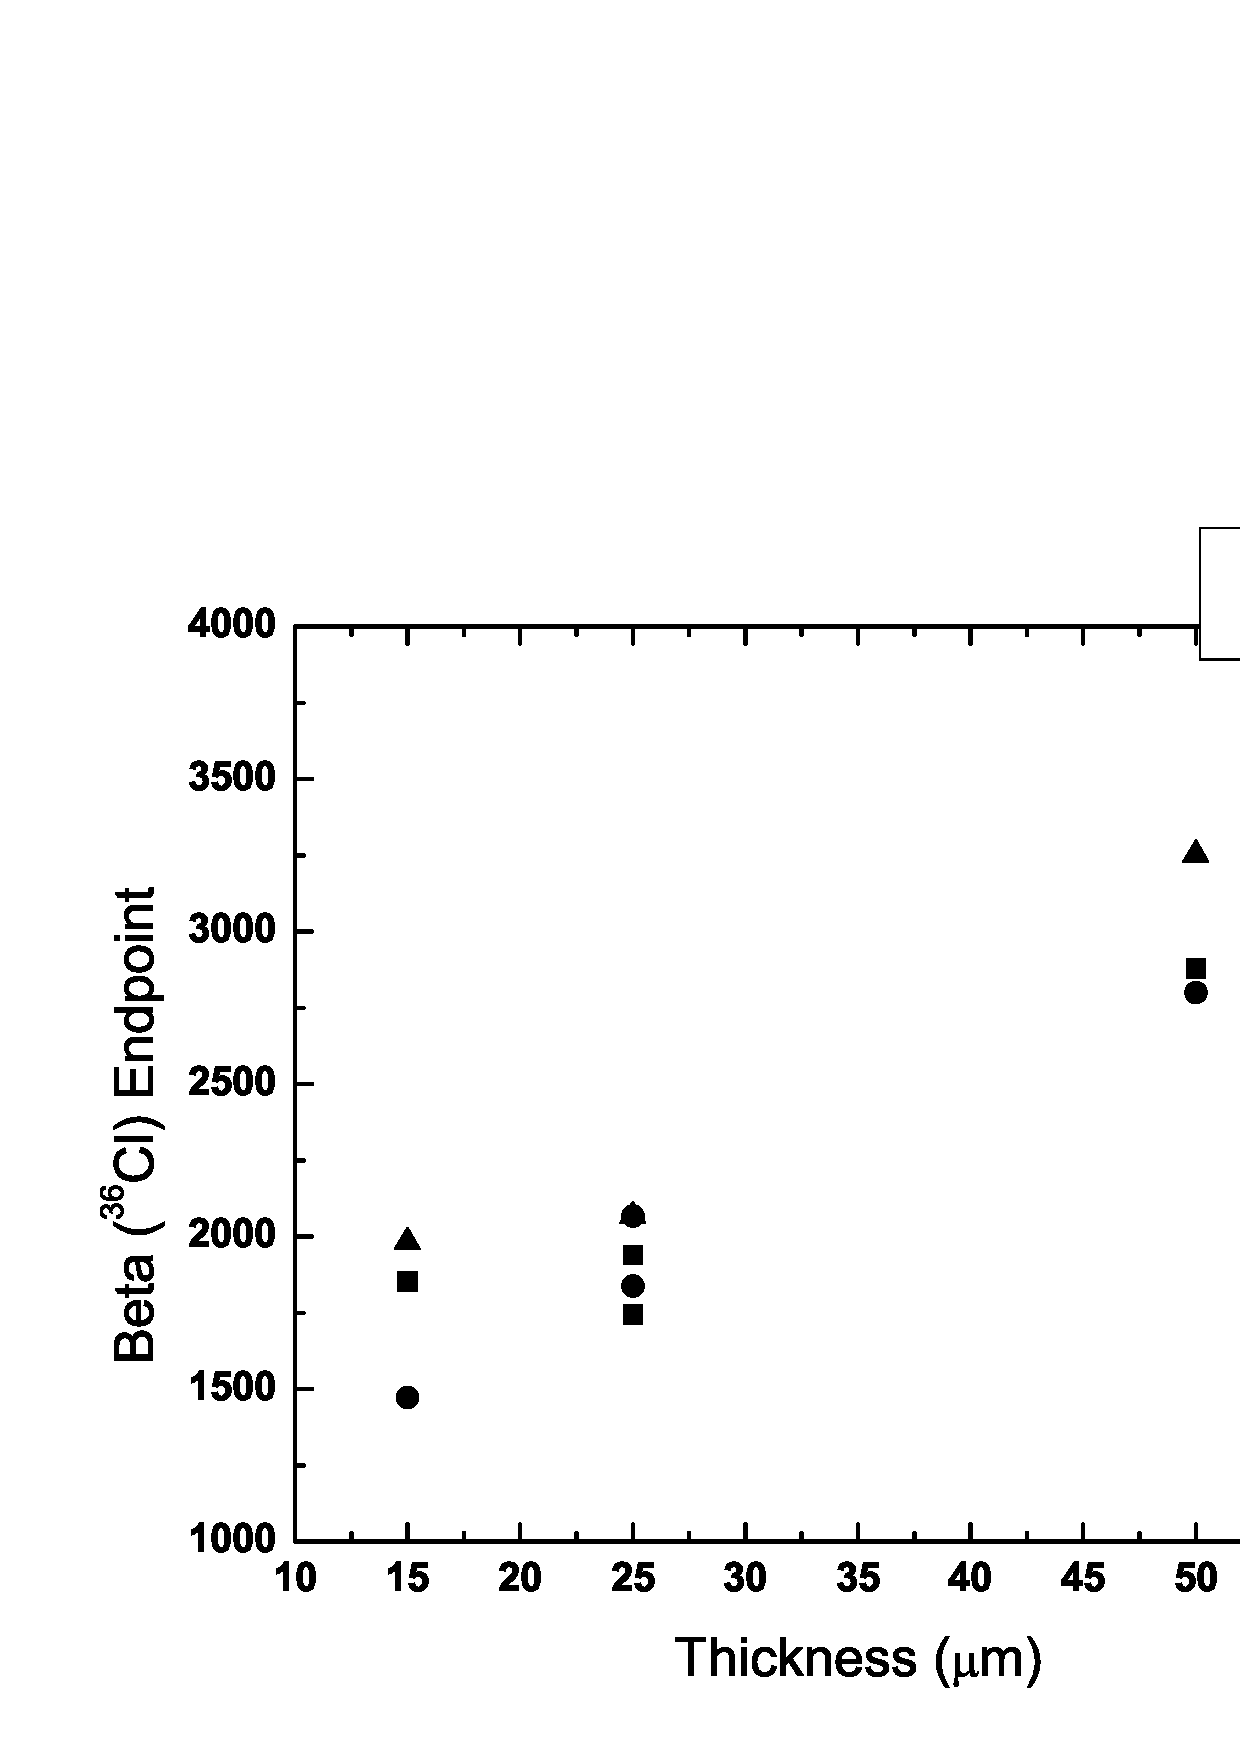
\includegraphics[width=\textwidth]{Beta}
        \caption{Beta Spectra Endpoints for a 5\% PS film}
    \end{subfigure}
    \begin{subfigure}[b]{0.45\figurewidth}
        \includegraphics[width=\textwidth]{PS-5PPOPOPOP_GammaAvg}
        \caption{Gamma Spectra Averages for PS films}
    \end{subfigure}
    \label{fig:SpectraFeatures}
\end{figure}
Figure \ref{fig:GammaIntrNeutronCounts} shows the intrinsic efficiency of these film (from spectra obtained from a \iso{Co}{60} source).
As the film thickness increases the pulse height discriminator at which an intrinsic efficiency of one in a million ($\epsilon_{int,\gamma} \le 10^{-6}$) is reached also increase.
The neutron spectra (shown in the solid lines) does not increase in light yield with increasing thickness, further providing an indication that the thickness of the films can be optimized to maximize the neutron count rates\footnote{The neutron count rate is increased with thickness by the increased mass of the detector} while minimizing the response of the detector to photons.
%%%%%%%%%%%%%%%%%%%% Figures %%%%%%%%%%%%%%%%%%%%%%%%
\begin{figure}
    \centering
    \caption{Gamma intrinsic efficiency (dashed lines) plotted against neutron counts (solid)}
    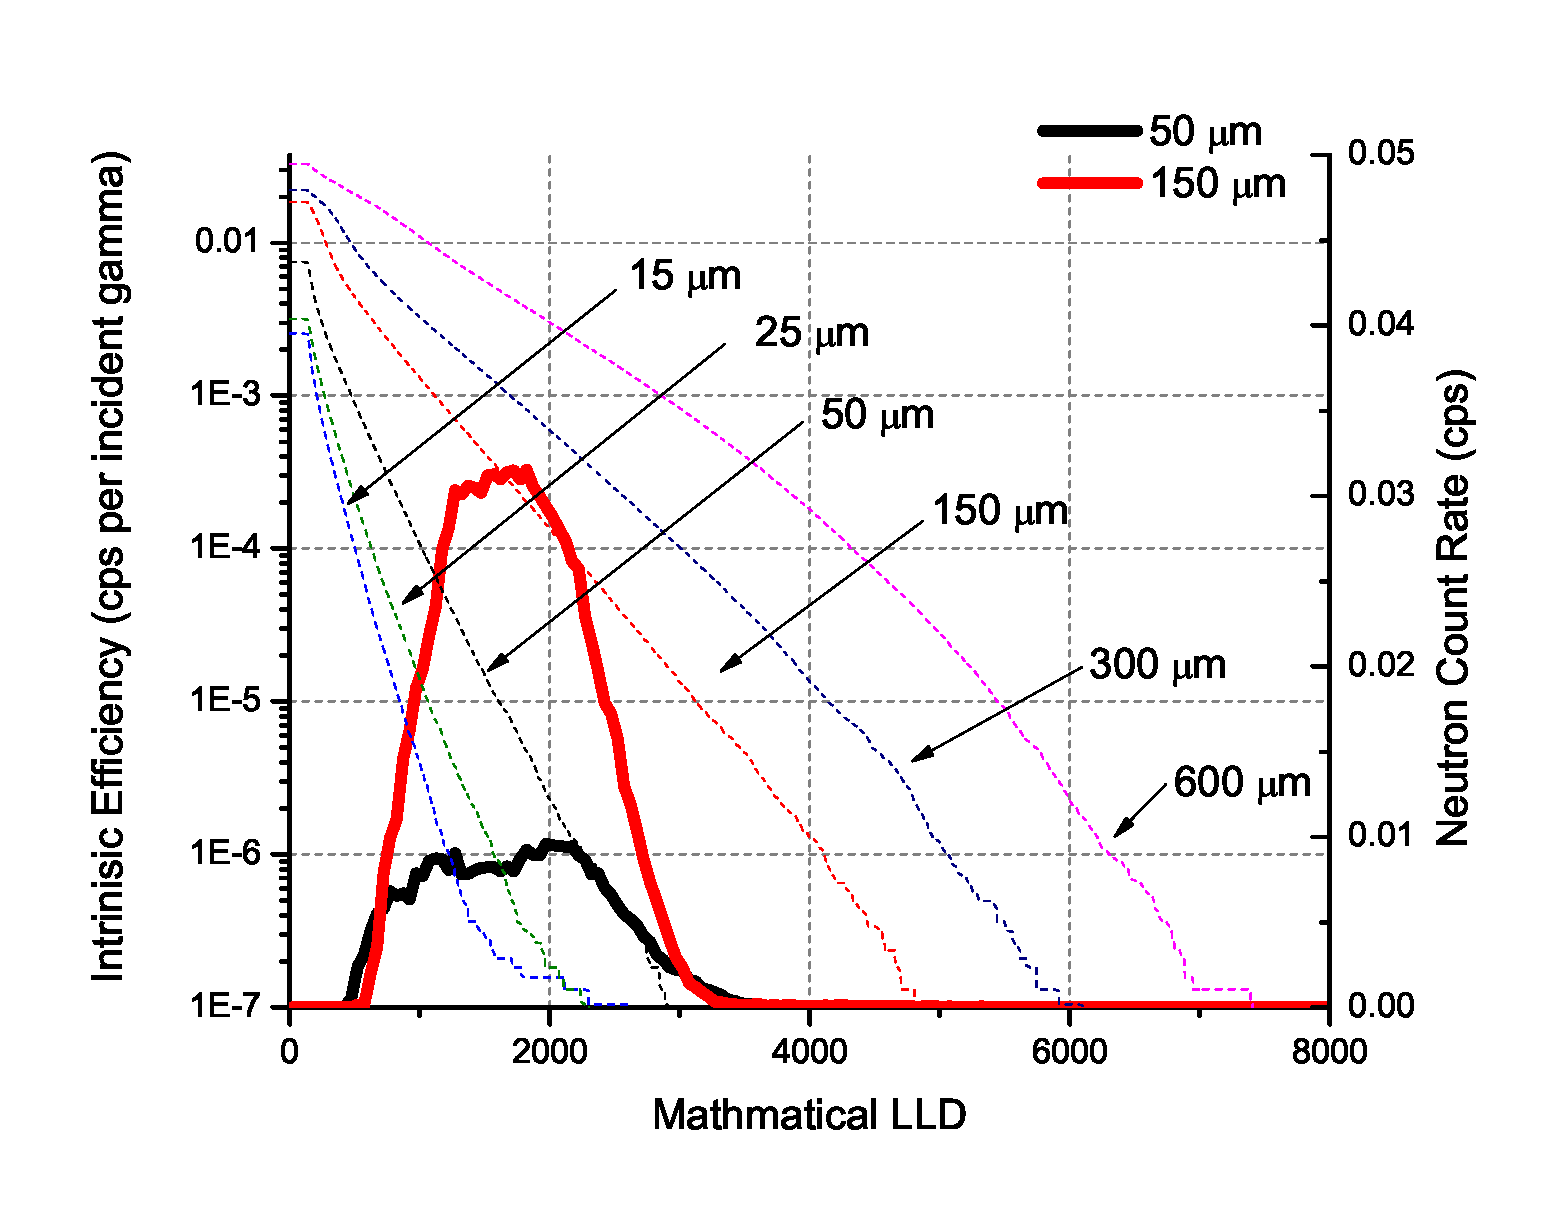
\includegraphics[width=\textwidth]{PS_IntEff_LiF20_PPO5}
    \label{fig:GammaIntrNeutronCounts}
\end{figure}


%%%%%%%%%%%%%%%%%%%%%%%%%%%%%%%%%%%%%
\section{Introduction to GEANT4}
\label{sec:G4Intro}

GEANT4 (GEomentry ANd Tracking) is a free, open source Monte Carlo based physics simulation toolkit developed and maintained at CERN widely used in the physics community.
As GEANT4 is a toolkit primarily developed for high energy physics particles are designated according the the \verb+PDG+ (Particle Data Group) encoding.
In addition, the physics processes are referenced according to the standard model.
In the standard model particles are divided into two families, bosons (the force carriers such as photons) and fermions (matter).
The fermions consist of both hadrons and leptons.
Hadrons are particles composed of quarks which are divided into two classes: baryons (three quarks) and mesons (two quarks).
Typical baryons include the neutron and the proton, while an example of a meson is the pion.
An example of a lepton is the electron.
\subsection{Organization of the GEANT4 Toolkit}
The GEANT4 toolkit is divided into eight (8) class categories:
\begin{itemize}
    \item Run and Event - generation of events and secondary particles.
    \item Tracking and Track - transport of a particle by analyzing the factors limiting the step size and by applying the relevant physics models.
    \item Geometry and Magnetic Field - the geometrical definition of a detector (including the computation of the distances to solids) as wells as the management of magnetic fields.
    \item Particle Definition and Matter - definition of particles and matter.
    \item Hits and Digitization - the creation of hits and their use for digitization in order to model a detectors readout response.
    \item Visualization - the visualization of a simulation including the solid geometry, trajectories and hits.
    \item Interface - the interactions between the toolkit and graphical user interfaces and well as external software.
\end{itemize}

There are then three classes which must be implemented by the user in order use the toolkit. These classes are:
\begin{itemize}
    \item \verb+G4VuserDetectorConstruction+ which defines the geometry of the simulation,
    \item \verb+G4VUserPhysicsList+ which defines the physics of the simulation, and
    \item \verb+G4VUserPriamryGeneratorAction+ which defines the generation of primary events.
\end{itemize}
Five additional classes are available for further control over the simulation:
\begin{itemize}
    \item \verb+G4UserRunAction+ which allows for user actions
\end{itemize}
\subsection{GEANT4 Tracking and Secondaries}
A GEANT4 simulation starts with a run which contains a set number of events.
An event is particular process of interest to the user, such as shooting a single particle at a detector. 
Typical usage might be to have a run be firing 1,000 neutrons at a detector, were each neutron is a single event.
Each particle transported in GEANT4 is assigned a unique track ID and a parent ID.
The particle that initiates the event is given a parent ID of 0 and a track ID of 1.
If the parent particle has a collision and produces a secondary particle this secondary particle is then given a parent ID of 1 (corresponding to the first secondary) and a track ID of 2.
Secondaries are tracked in GEANT4 utilizing a stack tracking the most recent secondary (and its cascade) first.
Listing \ref{lst:TrackingExample} provides an example from the verbose output of GEANT4 of the tracking in which only secondaries are not shown for the secondaries.
The initial particle in the event is the neutron because it has a parent ID of 0.
The alpha and triton are the secondaries produced by this collision. 
The alpha is assigned a parent ID of 1 (corresponding to the first generation) with a track ID of 3.
The triton is also assigned a parent ID of 1, but with a track ID of 2.
\begin{lstlisting}[language=,basicstyle=\tiny,caption={Tracking Example},label=lst:TrackingExample]
*********************************************************************************************************
* G4Track Information:   Particle = neutron,   Track ID = 1,   Parent ID = 0
*********************************************************************************************************

Step#    X(mm)    Y(mm)    Z(mm) KinE(MeV)  dE(MeV) StepLeng TrackLeng  NextVolume ProcName
    0        0        0    -6.59   2.5e-08        0        0         0    Absorber initStep
    1        0        0    -3.64         0        0     2.95      2.95    Absorber NeutronInelastic
    :----- List of 2ndaries - #SpawnInStep=  2(Rest= 0,Along= 0,Post= 2), #SpawnTotal=  2 ---------------
    :         0         0     -3.64      2.73             triton
    :         0         0     -3.64      2.05              alpha
    :----------------------------------------------------------------- EndOf2ndaries Info ---------------

*********************************************************************************************************
* G4Track Information:   Particle = alpha,   Track ID = 3,   Parent ID = 1
*********************************************************************************************************

Step#    X(mm)    Y(mm)    Z(mm) KinE(MeV)  dE(MeV) StepLeng TrackLeng  NextVolume ProcName
    0        0        0    -3.64      2.05        0        0         0    Absorber initStep
    1 -0.000201 0.000128    -3.64      2.01   0.0491 0.000266  0.000266    Absorber ionIoni
    2 -0.00049 0.000312    -3.64      1.93   0.0705 0.000381  0.000647    Absorber ionIoni

*********************************************************************************************************
* G4Track Information:   Particle = triton,   Track ID = 2,   Parent ID = 1
*********************************************************************************************************

Step#    X(mm)    Y(mm)    Z(mm) KinE(MeV)  dE(MeV) StepLeng TrackLeng  NextVolume ProcName
    0        0        0    -3.64      2.73        0        0         0    Absorber initStep
    1 0.000339 -0.000215    -3.64      2.71   0.0116 0.000447  0.000447    Absorber hIoni
\end{lstlisting}



%%%%%%%%%%%%%%%%%%%%%%%%%%%%%%%%%%%%%
\section{Methods}
\label{sec:Methods}

For convince a subversion repository was created to manage the developed code base, and all source code is available by anonymous checkout from \verb+http://www.murphs-code-repository.googlecode.com/svn/trunk/layeredPolymerTracking+. Revision 360 was the code base used to generate the results shown in \ref{sec:Results}.

\subsubsection{Detector Geometry}
The geometry was setup such that it is possible to define multiple layers of detectors, as shown in Figure \ref{fig:LayerDetectorGeo}.
This was done by creating a 
\begin{figure} 
    \includegraphics[width=\figurewidth]{10LayerGamma}
	\caption{10 Layer Detector with a simulated gamma event}
    \label{fig:LayerDetectorGeo}
\end{figure}
\subsubsection{Physics Lists}

%%%%%%%%%%%%%%%%
\section{Simulation Validation}
\label{sec:SimValidation}

GEANT4 is a toolkit implemented by the user so extensive efforts were completed in order to validate the results and ensure no bugs exists.
First steps were taken (for small runs) to compute the energy deposition for small runs by hand in order to make sure they agreeded with the analysis code.
In addition the reaction products of the \iso{Li}{6}$(\text{n},\alpha)$\iso{H}{3} were checked to make sure that they agreeded with the published values \footnote{GEANT4 4.9.2.p01 contains an error in which extra photons are generated, \hyperref{http://hypernews.slac.stanford.edu/HyperNews/geant4/get/phys-list/530.html}{SLAC hypernews}. This has been fixed in the release used, 4.9.5p1}.
The GEANT4 simulation was validated by comparing the single collision energy loss spectra in water and by comparing the simulation energy deposition to that of a measured spectra.


\subsection{Energy Deposition Validation}
The energy deposition was tested by reproducing the single collision energy loss spectra in water\footnote{%
An analysis class was not written for this simulation. 
Instead the verbosity of the simulation was set to \texttt{verbose=1} in the run macro.
The first ionisation collision (\texttt{e-\_G4DNAIonisation}) was then extracted with \texttt{sed -n '/ParentID = 0/,/e-\_G4DNAIonisation/p' G4OutputFileName.txt| grep "e-$\backslash$\_G4DNAIonisatioin" | awk '\$\{print \$5\}' }' %
}.
The \verb+PhysicsList+ was extended to include \verb+G4DNAPhysics+ and the detector material was set to the NIST definition contained in the toolkit with \verb+G4Material* H20 = man->FindOrBuildMaterial("G4_WATER")+.
In general there was excellent agreement between the simulated energy spectra and a previously published spectra\cite{turner_comparative_1982}.
The simulated spectra had much better resolution at fine energies (corresponding to discrete states) of which Turners did not.
%%%%%%%%%%%%%%%%%%%% Figures %%%%%%%%%%%%%%%%%%%%%%%%
\begin{figure}[h]
    \centering
    \begin{subfigure}[b]{0.45\figurewidth}
        \includegraphics[width=\textwidth]{SingleCollisionEnergyLoss_300bins}
        \caption{Simulated}
    \end{subfigure}
    \begin{subfigure}[b]{0.45\figurewidth}
        \includegraphics[width=\textwidth]{Turner_Fig2_SingleCollisionELoss}
        \caption{Single-collision energy loss spectra for electrons in water \protect\cite{turner_comparative_1982}}
        \caption{Published}
    \end{subfigure}
    \caption{Single Collision Energy Loss of Water}
\end{figure}
\subsection{Spectra Validation}
The simulated energy deposition is not the directly equivilant to light collected on the PMT because the scintillation process and light collection is not modeled.
However, it is well known that scintillation follows the energy deposition\cite{birks_scintillations_1951}.
Thus, up to scaling contants, the energy deposition can be considered equivilant to the scintillation and representative of the measured spectra.
Rather than attempting to back out these scaling contants the weighted average of spectra were used in which integration and normalization removes these fudge factors.
The simulation was validated by computing the weighted average of the energy deposition \ref{eq:AvgEnergyDepDefination} and comparing it to the spectra average defined in \ref{eq:AvgChannelNumberDefination}.
There is excellent agreement between the measured gamma weighted average (right ordinate axis) and the average energy deposition from a \iso{Co}{60} source (left ordinate axis).
Non-linearity is observed for films less than 200 \micron, this is evidance that the cascade electrons from the Compton electron are eneregetic enough that the range of the electrons is much greater than the thickness of the film and leave the film without colliding to an energy in which the energy deposition is linear (Figure ~\ref{fig:TurnerETransfer}).
%%%%%%%%%%%%%%%%%%%%% Equations %%%%%%%%%%%%%%%%%%%%%%
\begin{equation}
\label{eq:AvgEnergyDepDefination}
<E> = \frac{\int_0^\infty {\phi(E)EdE}}{\int_0^\infty{\phi(E)dE}} \\
\text{where}
\end{equation}
\begin{equation}
\label{eq:AvgChannelNumberDefination}
<\mu> = \frac{\int_0^\infty {f(x)xdx}}{\int_0^\infty{x(x)dx}} \\
\text{where}
\end{equation}
%%%%%%%%%%%%%%%%%%%% Figures %%%%%%%%%%%%%%%%%%%%%%%%
\begin{figure}
    \centering
    \caption{Gamma Simulation Agreement}
    \includegraphics[width=\textwidth]{G4EDep_LightYield_Co60}
    \label{fig:GammaSimAgreement}
\end{figure}
\begin{figure}
    \centering
    \caption{Neutron Simulation Agreement}
    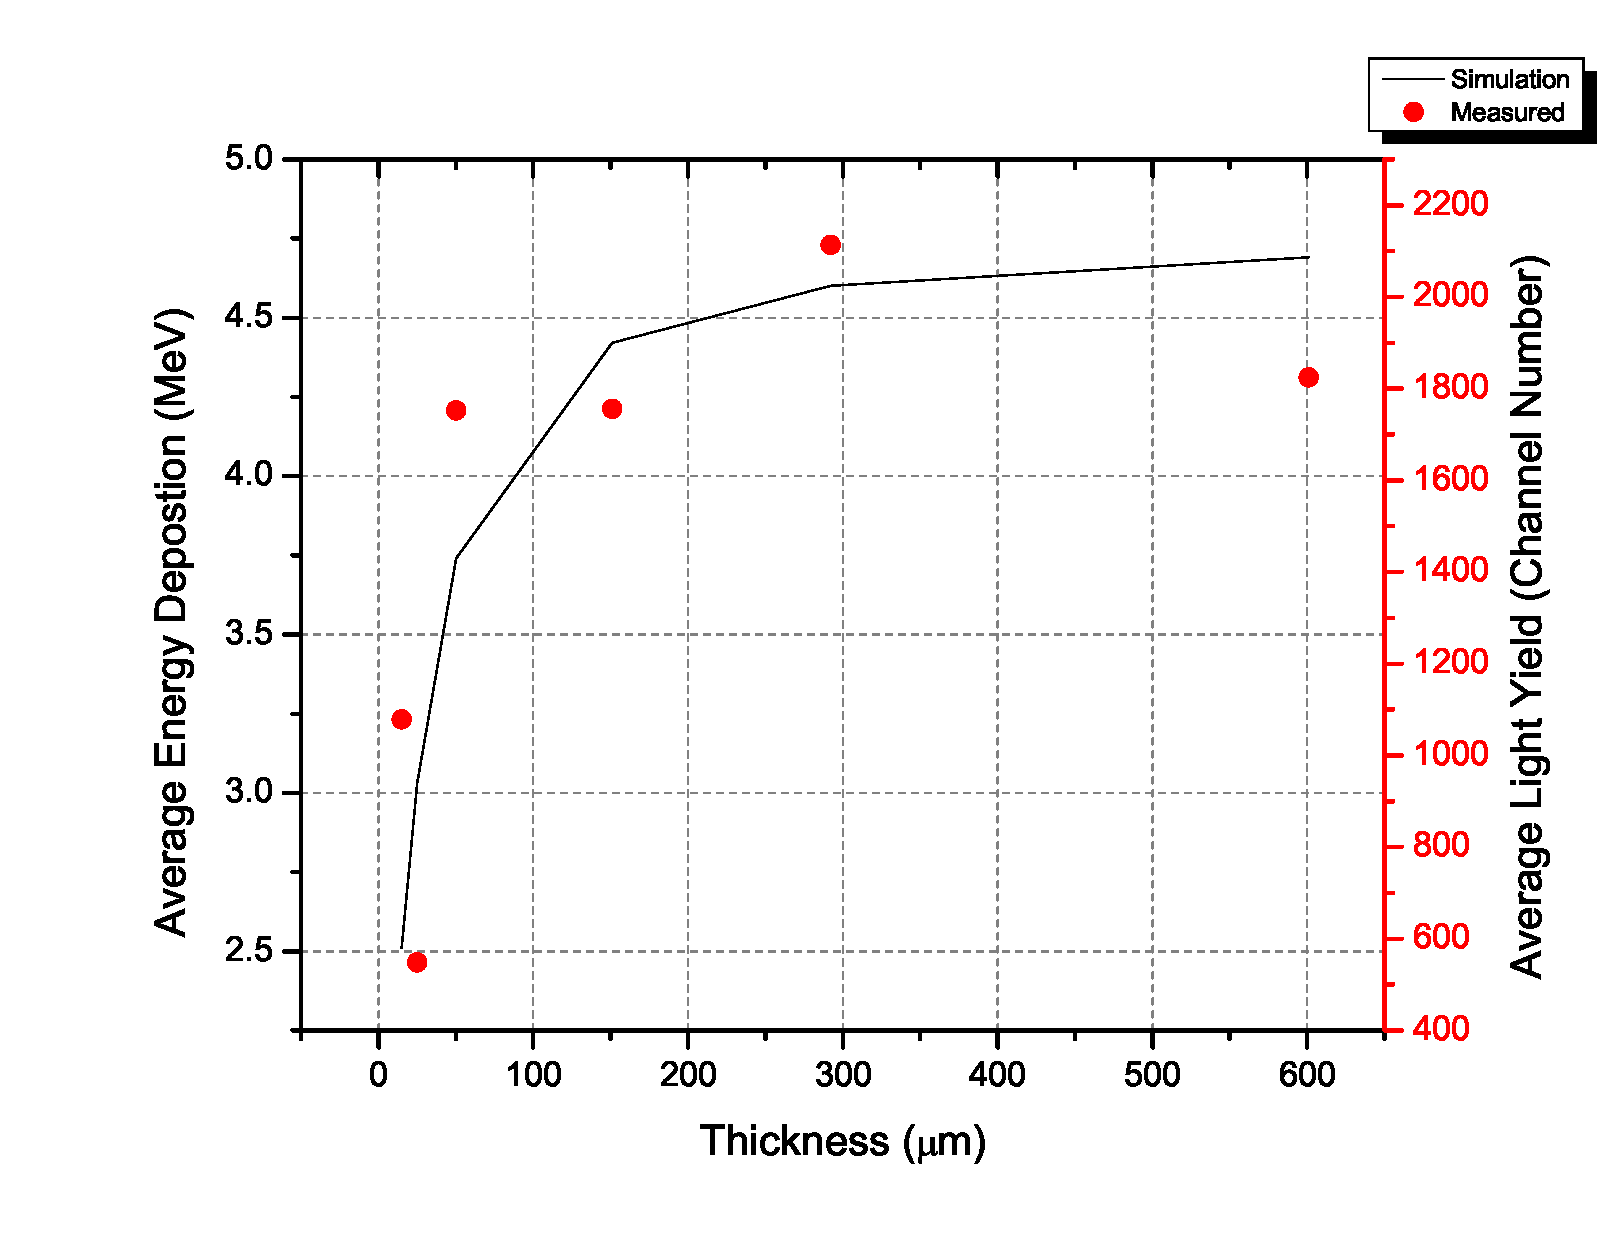
\includegraphics[width=\textwidth]{G4EDep_LightYield_Neutron}
    \label{fig:NeutronSimAgreement}
\end{figure}

The comparison between the average energy deposition and measured channel allows for the a relationship to be drawn between the energy deposited and the channel number.
This is completed by an taking an average of the ratio between the average channel number (Equation \ref{eq:AvgChannelNumberDefination} and the average energy deposition (Equation \ref{eq:AvgEnergyDepDefination}).
This ratio is defined in Equation \ref{eq:ChannelNumber}.  This quantity is defined seperately for neturons and gammas.
%%%%%%%%%%%%%%%%%%%%% Equations %%%%%%%%%%%%%%%%%%%%%%
\begin{equation}
\label{eq:ChannelNumber}
\eta = \sum_t { \frac{<E>}{<\mu}} 
\end{equation}

\section{Results}
\label{sec:Results}

\subsection{Parmater Search}

The parameter search for the optimal C and $\sigma$ parameters is shown in the contour plots of Figures \ref{fig:ParamLiver}, \ref{fig:ParamGlass} and \ref{fig:ParamGlass}.
The optimal classifier parameters are shown for the coarse parameter search in Table \ref{tab:CoarseParamValues} and for the fine parameter search in Table \ref{tab:FineParamValues}.
\todo{Make some quantifications and discuss the data}
\begin{table}[h!]
\caption{Coarse Optimal Classifier Parameters}
\label{tab:CoarseParamValues}
\begin{tabular}{c c c c c c c c}
\hline
Data Set & $C_{min}$ & $C_{max}$ & $\sigma_{min}$ & $\sigma_{max}$ & $C$ & $\sigma$ & $\epsilon$ \\ 
\hline
Glass & -5.00 & 5.00 & -5.00 & 5.00 & 5.00 & 0.56 & 72.78 \\ 
Liver & -5.00 & 5.00 & -5.00 & 5.00 & 3.89 & -2.78 & 74.33 \\ 
Vowel & -5.00 & 5.00 & -5.00 & 5.00 & 5.00 & 2.78 & 99.24 \\ 
\hline
\end{tabular}
\end{table}
\begin{table}[ht]
\caption{Fine Optimal Classifier Parameters}
\label{tab:FineParamValues}
\begin{tabular}{c c c c c c c c}
Data Set & $C_{min}$ & $C_{max}$ & $\sigma_{min}$ & $\sigma_{max}$ & $C$ & $\sigma$ & $\epsilon$ \\ 
\hline
Glass & 2.50 & 7.50 & 0.28 & 0.83 & 6.71 & 0.31 & 75.00 \\ 
Liver & 1.94 & 5.83 & -4.17 & -1.39 & 3.79 & -1.68 & 75.67 \\ 
Vowel & 2.50 & 7.50 & 1.39 & 4.17 & 7.50 & 1.97 & 99.43 \\ 
\hline
\end{tabular}
\end{table}
\begin{figure*}[ht!]
	\centering
	\begin{subfigure}[b]{0.45\textwidth}
		\centering
		\includegraphics[width=\textwidth]{Liver_coarseSearch}
        \caption{Coarse Search}
	\end{subfigure}%
	~
	\begin{subfigure}[b]{0.45\textwidth}
		\centering
		\includegraphics[width=\textwidth]{Liver_fineSearch}
        \caption{Fine Search}
	\end{subfigure}	
	\caption{Parameter search for Liver Disorder}
	\label{fig:ParamLiver}

	\begin{subfigure}[b]{0.45\textwidth}
		\centering
		\includegraphics[width=\textwidth]{Glass_coarseSearch}
        \caption{Coarse Search}
	\end{subfigure}%
	~
	\begin{subfigure}[b]{0.45\textwidth}
		\centering
		\includegraphics[width=\textwidth]{Glass_fineSearch}
        \caption{Fine Search}
	\end{subfigure}	
	\caption{Parameter search for Glass Disorder}
	\label{fig:ParamGlass}

	\begin{subfigure}[b]{0.45\textwidth}
		\centering
		\includegraphics[width=\textwidth]{Vowel_coarseSearch}
        \caption{Coarse Search}
	\end{subfigure}%
	~
	\begin{subfigure}[b]{0.45\textwidth}
		\centering
		\includegraphics[width=\textwidth]{Vowel_fineSearch}
        \caption{Fine Search}
	\end{subfigure}	
	\caption{Parameter search for Vowel Disorder}
	\label{fig:ParamVowel}
\end{figure*}

\subsection{AdaBoostM1}

\end{document}

